\documentclass[12pt]{iopart}
%\newcommand{\gguide}{{\it Preparing graphics for IOP Publishing journals}}
%Uncomment next line if AMS fonts required
%\usepackage{iopams}  
\usepackage[utf8]{inputenc}
\usepackage[T1]{fontenc}
\usepackage{biblatex} %Imports biblatex package
\usepackage{lineno}
\usepackage{graphicx}
\linenumbers

\addbibresource{sample.bib}

\begin{document}

\title[An Open Source Perovskite Solar Cell Passive Curve Tracer]{An Open Source Perovskite Solar Cell Passive Curve Tracer}

\author{Walker S. Arce}
\address{University of Nebraska-Lincoln, Department of Electrical and Computer Engineering, Lincoln, 68588, United States}
\ead{wsarcera@gmail.com}
\vspace{10pt}

\begin{indented}
\item[]September 2025
\end{indented}

\begin{abstract}
When developing systems for perovskite solar cells, it's important to have a testing platform that closely resembles your deployed systems.  While developing a 1U CubeSat, the Big Red Sat-1, at the University of Nebraska-Lincoln, we found a lack of passive curve tracing instrumentation, which we needed for our mission.  To that end, we developed a benchtop passive curve tracer that leverages the Ossila Solar Simulator as an AM1.0 light source.  This device utilizes a ladder of switched resistors and a precision voltage and current measurement to achieve the curve tracing.  It also integrates a common-anode multiplexer to switch through multi-pixel perovskite solar cells.  Finally, the solar cell holder is separate from the main measurement system, so various substrates sizes and pixel counts can be supported.  This system is tested using various perovskite solar cells.  It has been open sourced to enable reuse in future systems that may benefit from the lower power consumption and flight heritage.
\end{abstract}

\section*{Introduction}

A curve tracer performs a sweep of load conditions to assess how voltage and current vary accordingly.  These two variables are plotted with voltage on the x-axis and current on the y-axis, yielding a variety of common shapes.  Varying the load can be accomplished in many ways, such as using a MOSFET in the triode region, a potentiometer, or using a buck converter \cite{morales2021review}.  

Considering this project was completed for the Big Red Sat-1 mission, we prioritized low-power operation, low-voltage operation, and compact layout for a 1U CubeSat.  The other important aspect is the ability to switch through the multiple pixels that are built onto the substrate.

\section*{Methods}

\subsection*{Curve Tracer}

\subsection*{Common-Anode Multiplexer}

\section*{Results}

\subsection*{Hardware}

\subsection*{Software}

\begin{figure}[ht]
	\centering
	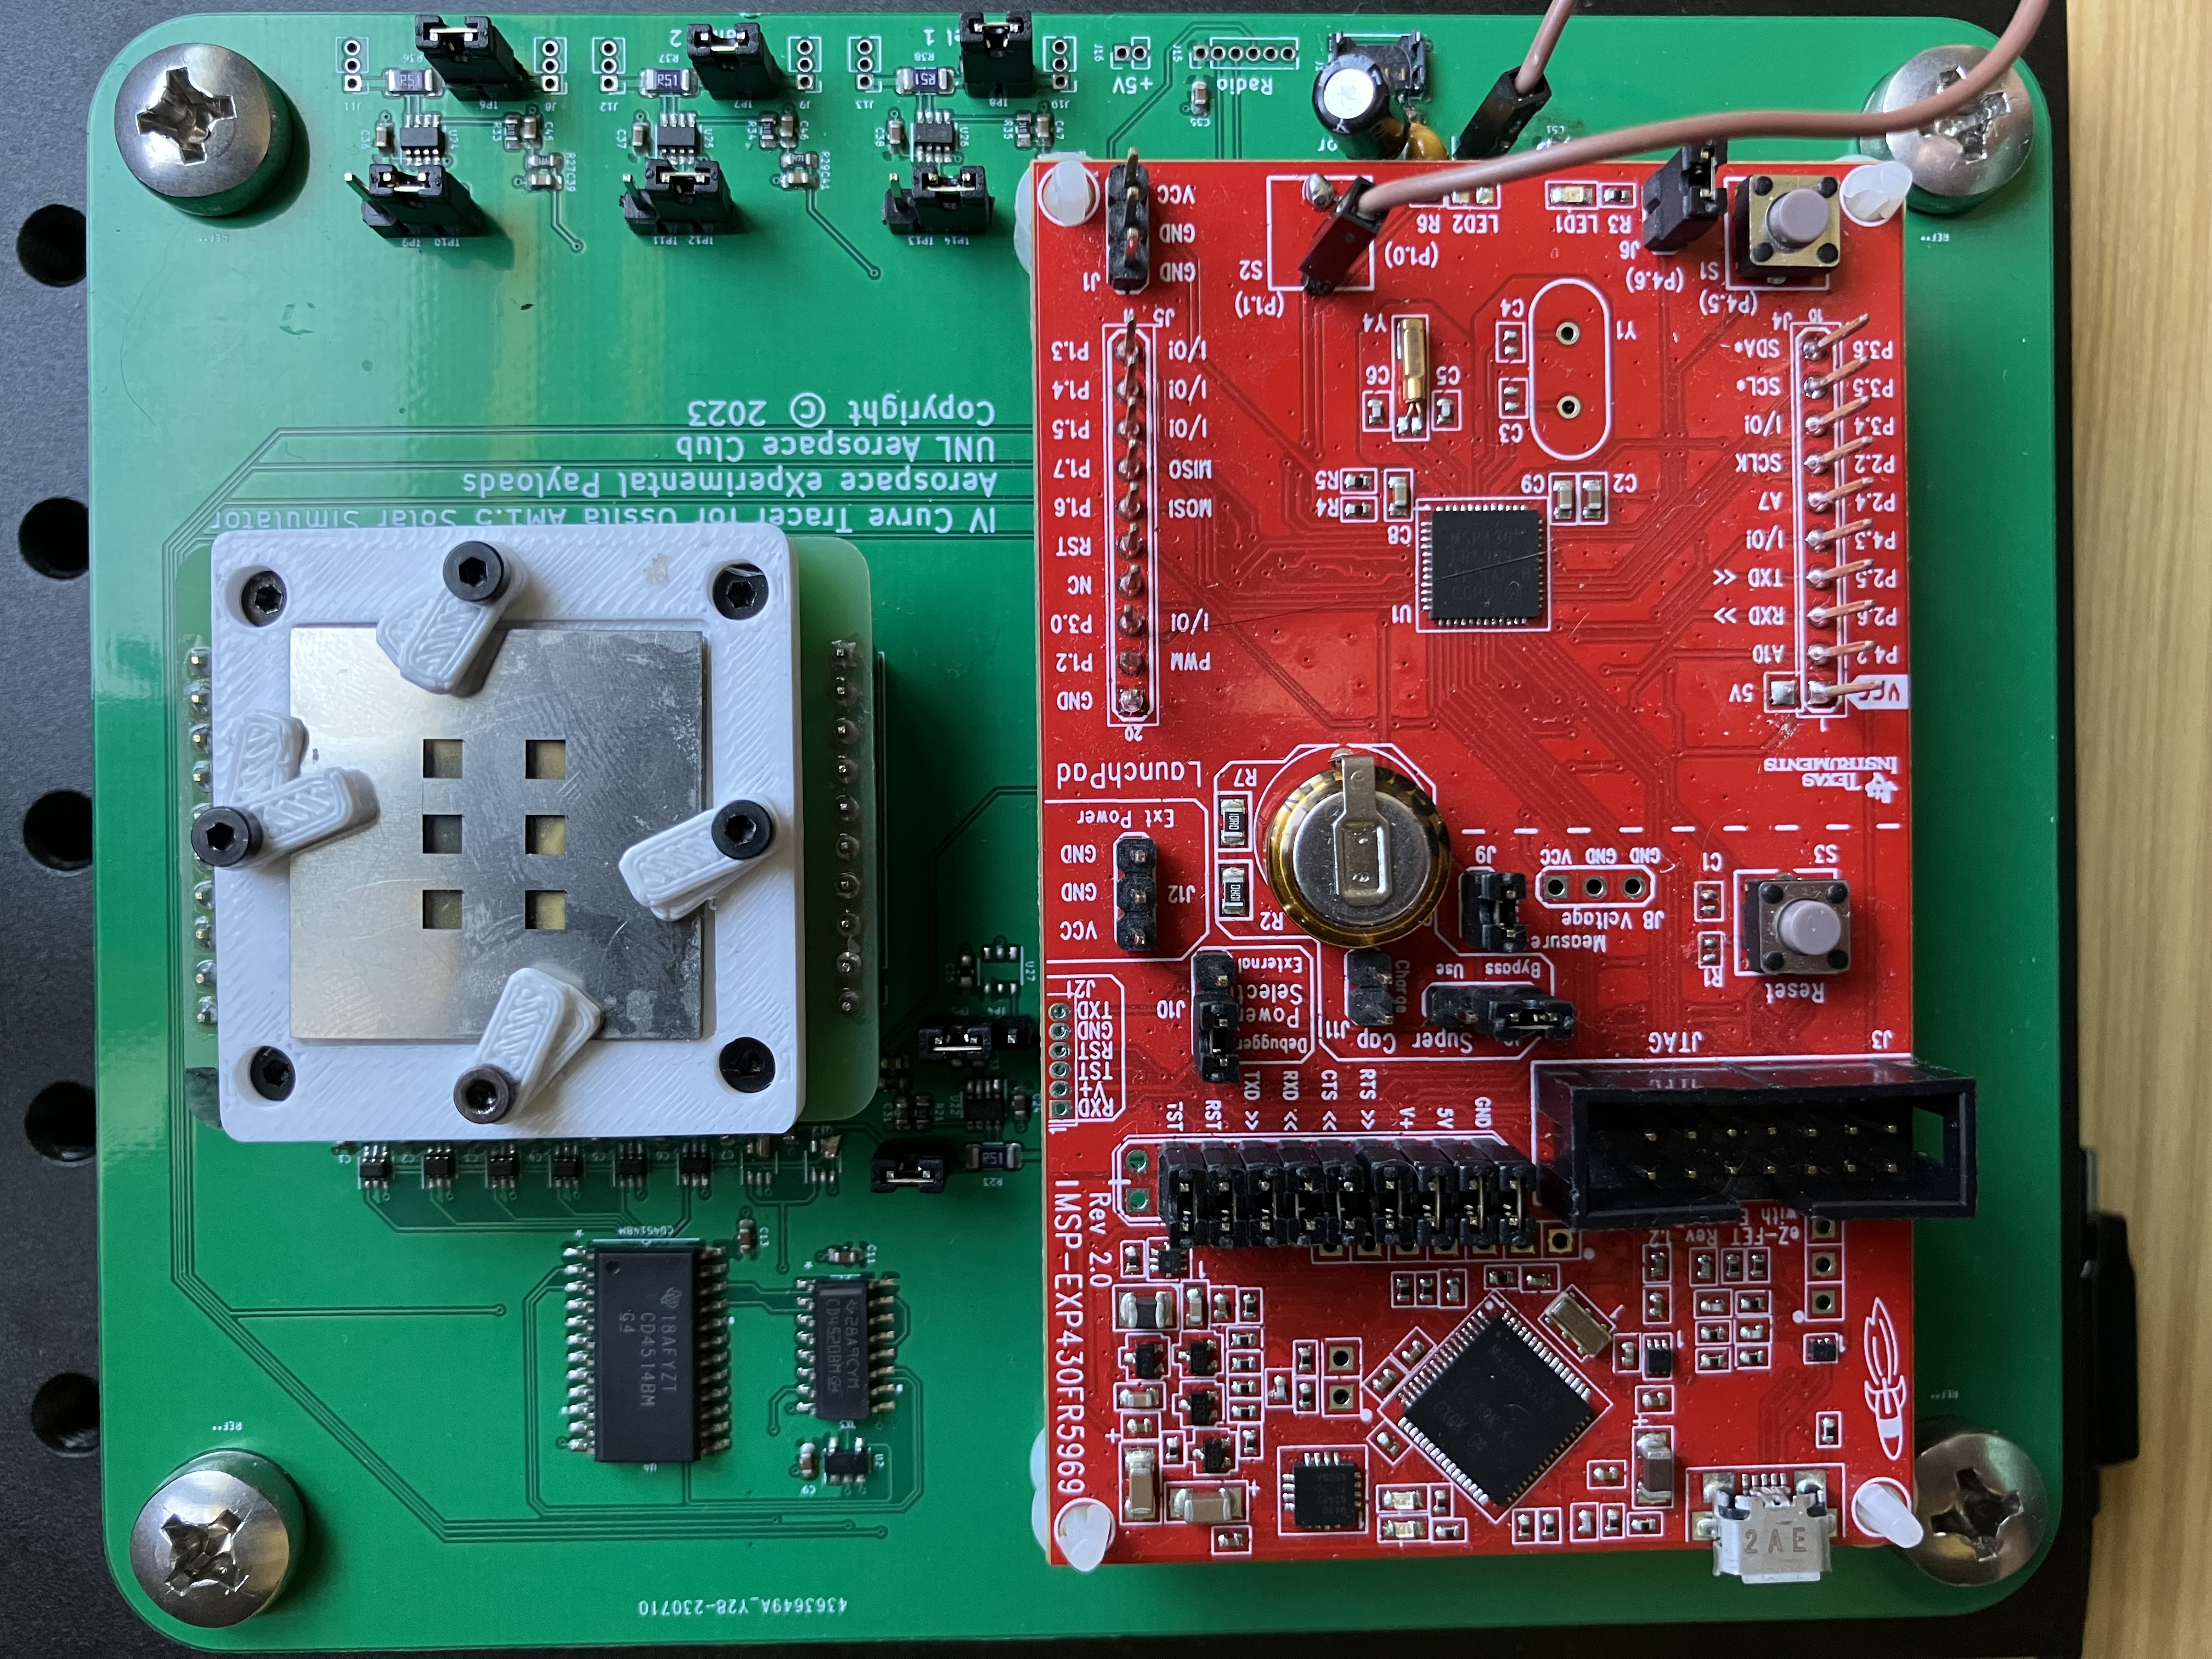
\includegraphics[width=\linewidth]{IMG_1317.jpg}
	\caption{The assembled curve tracer with a perovskite solar cell installed with light mask.}
	\label{fig:hardware}
\end{figure}

\begin{figure}[ht]
	\centering
	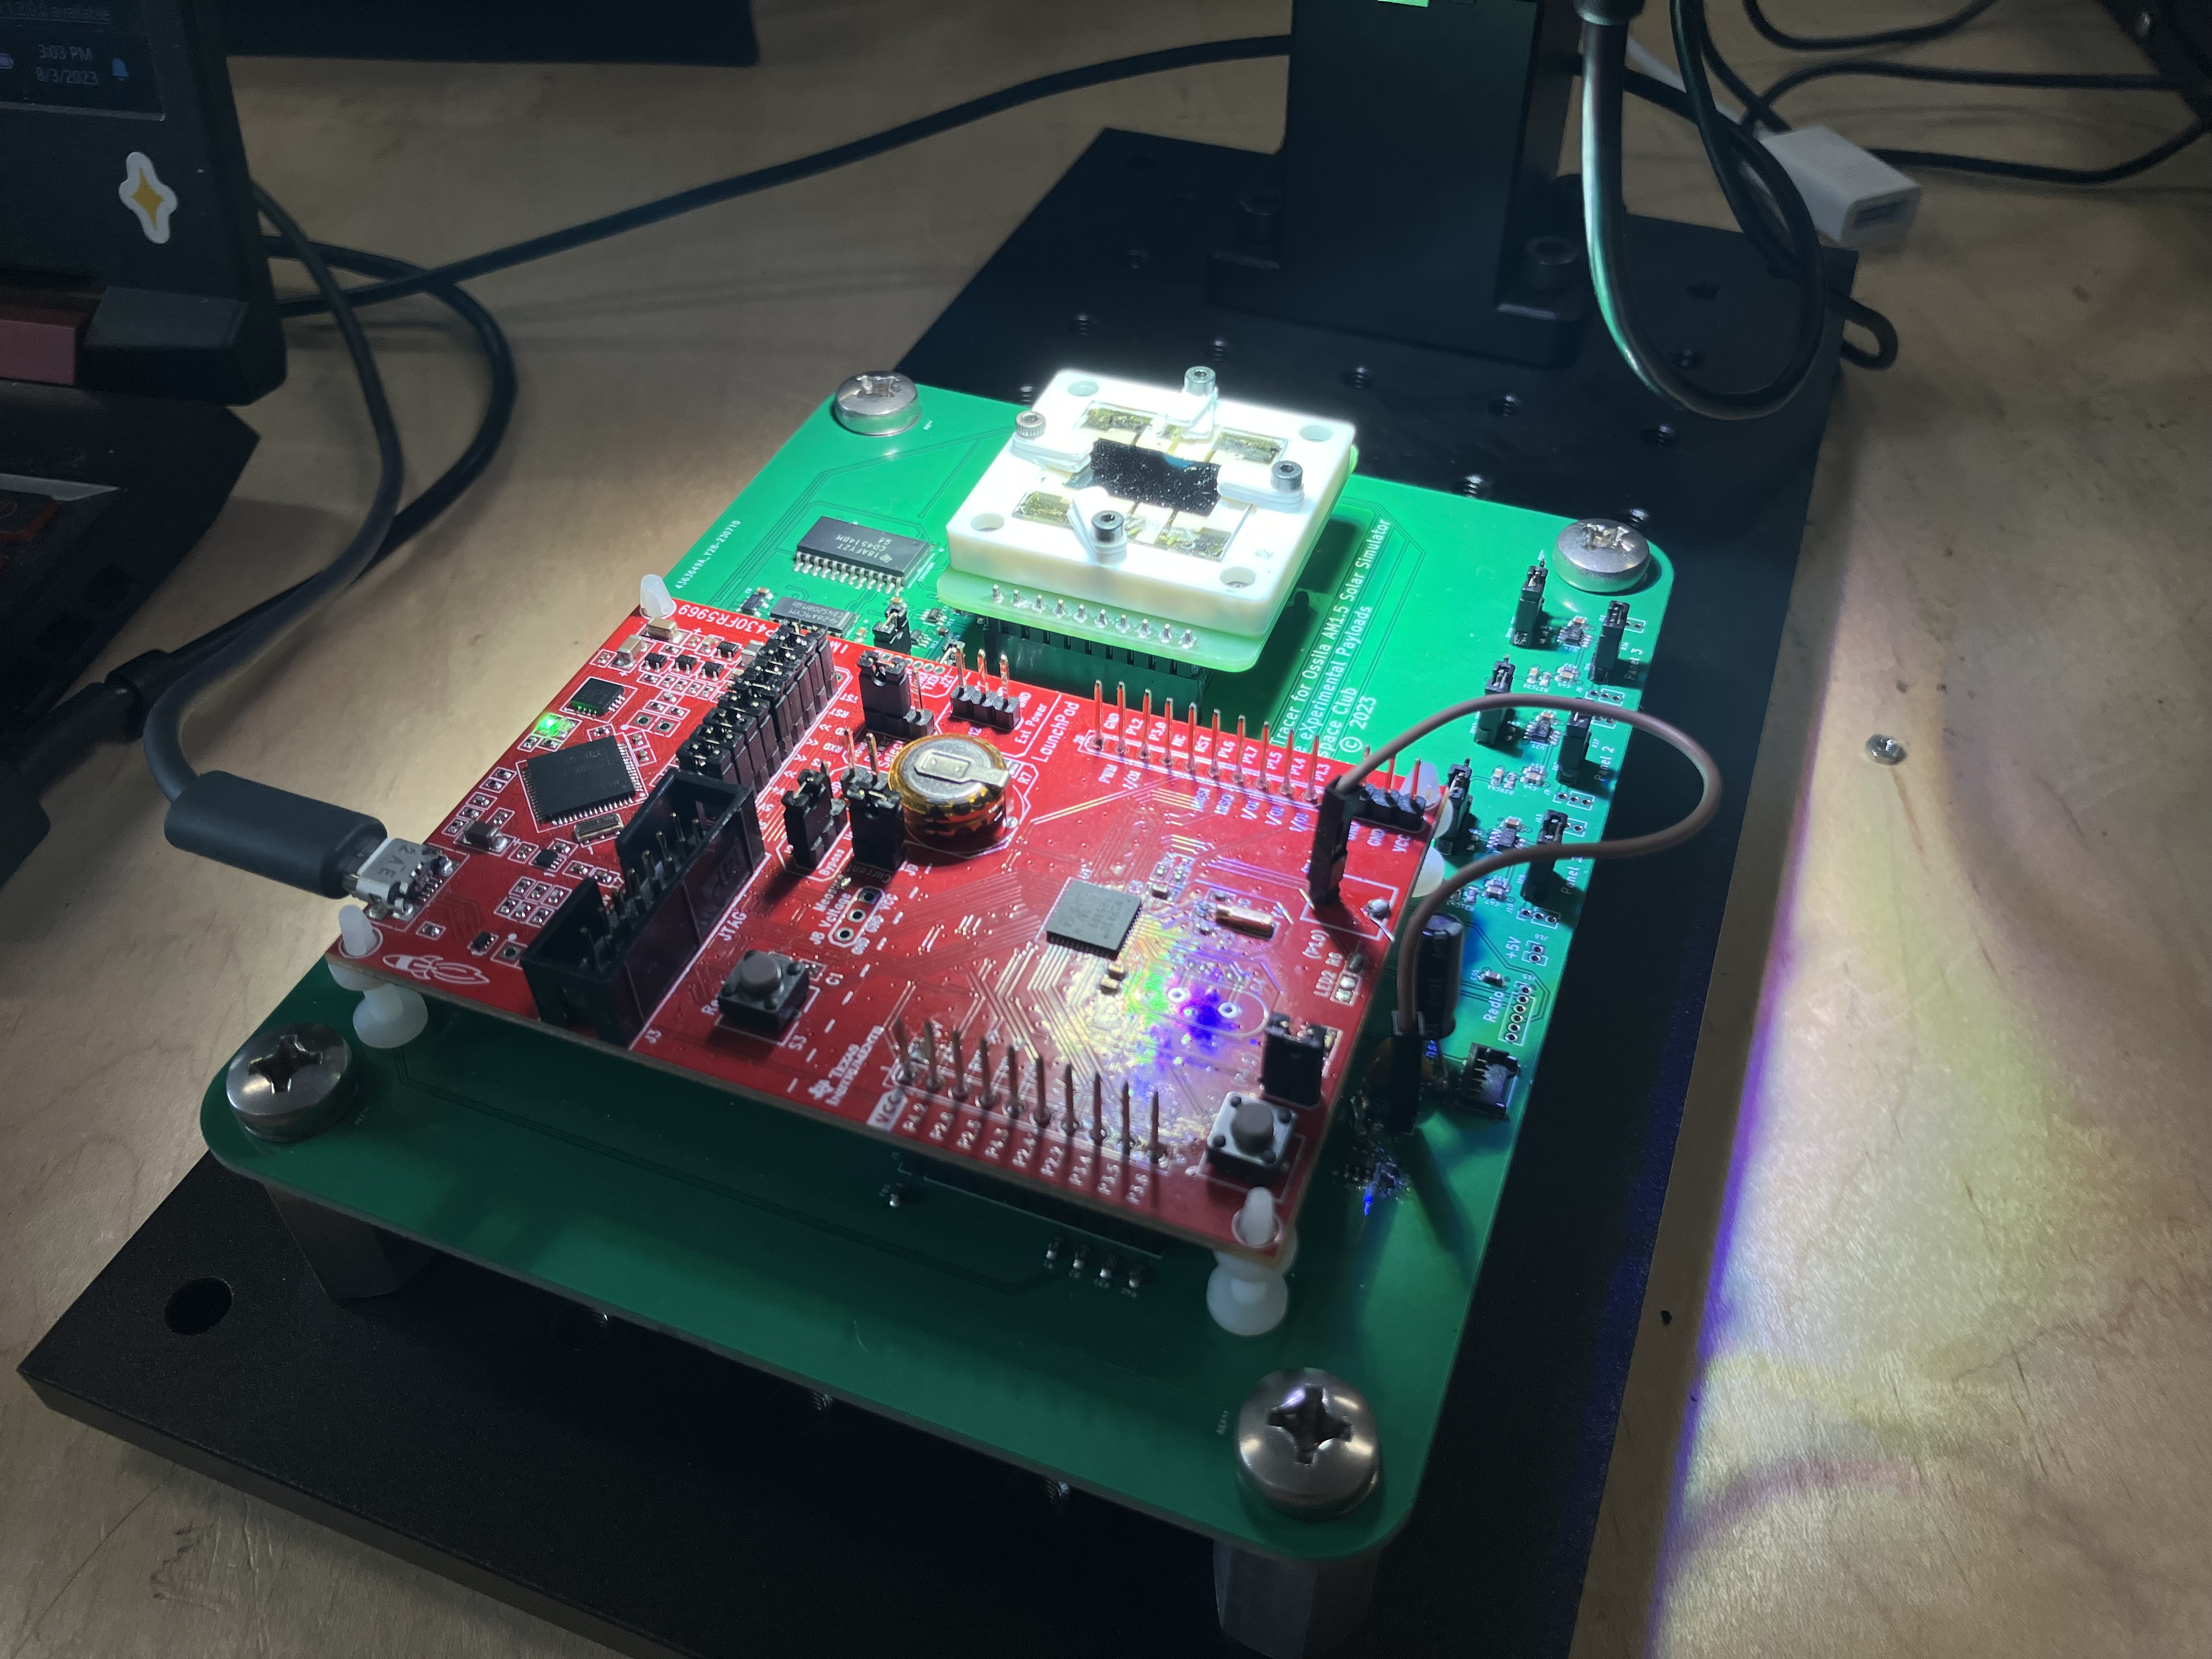
\includegraphics[width=\linewidth]{in use.jpg}
	\caption{The curve tracer in use with the Ossila solar simulator illuminating the sample.}
	\label{fig:inuse}
\end{figure}


\begin{figure}[ht]
	\centering
	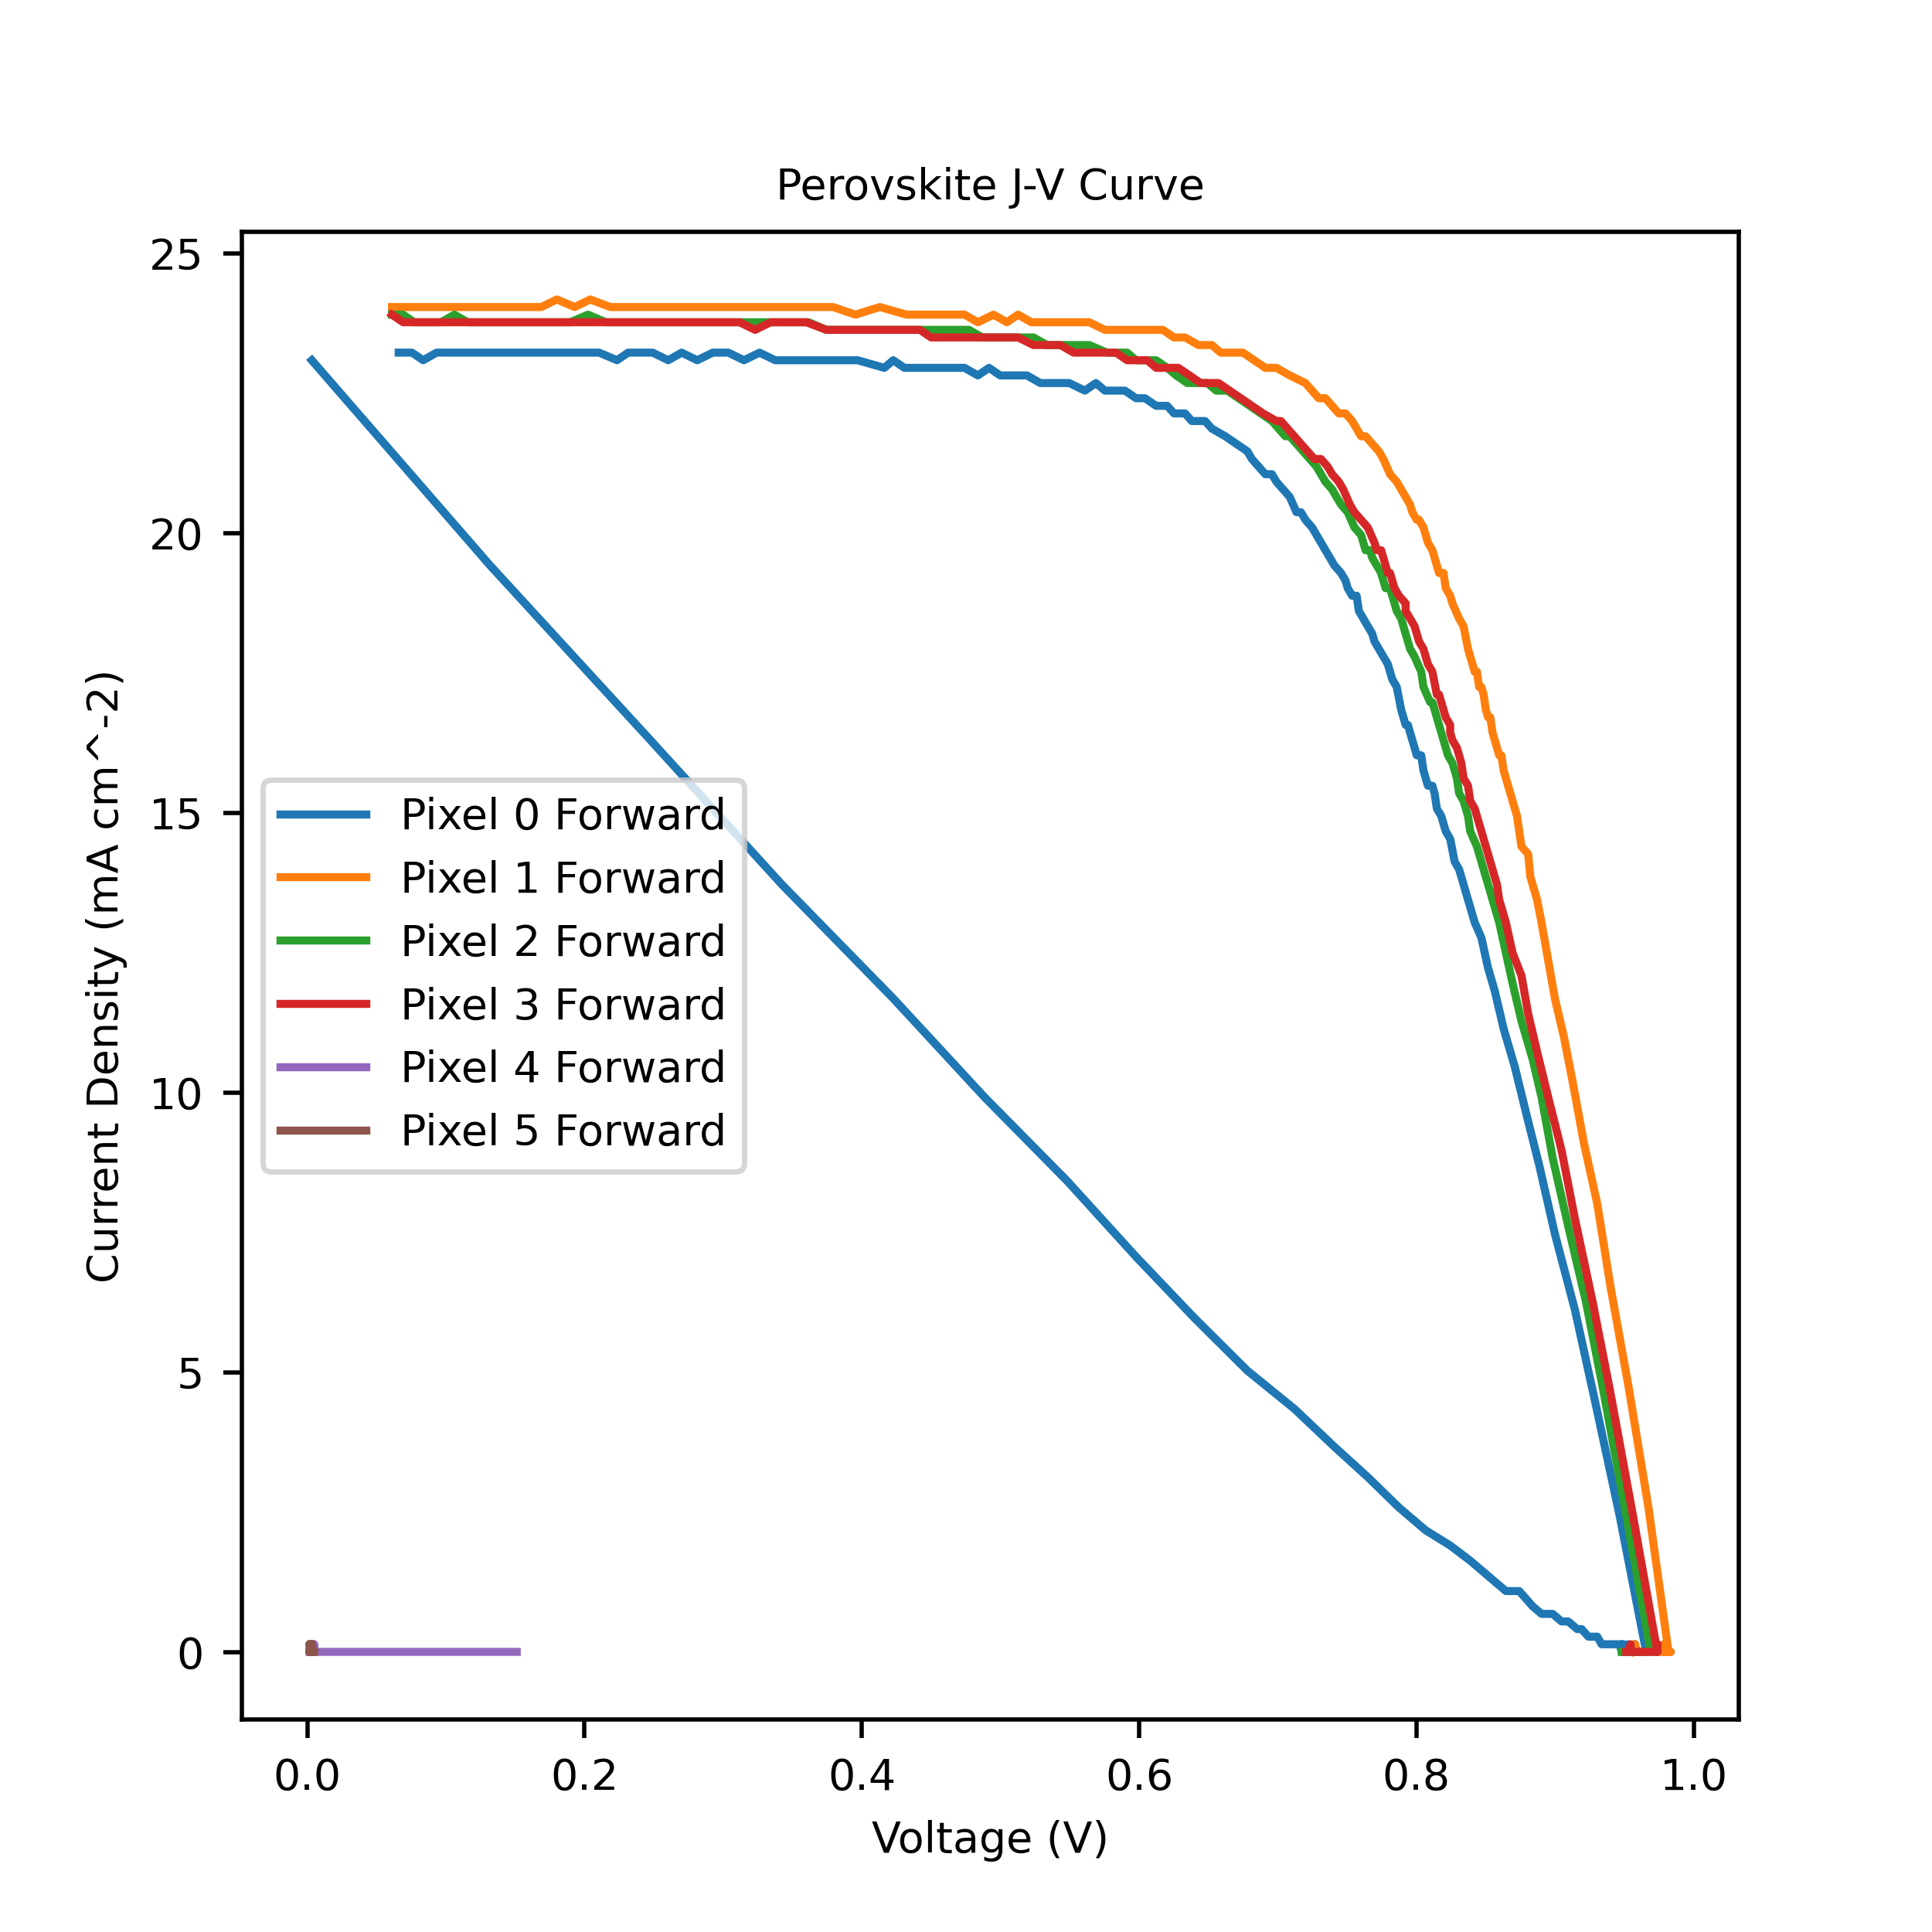
\includegraphics[width=7.5cm, height=7.5cm]{X017_LM_plotted_Forward.png}
	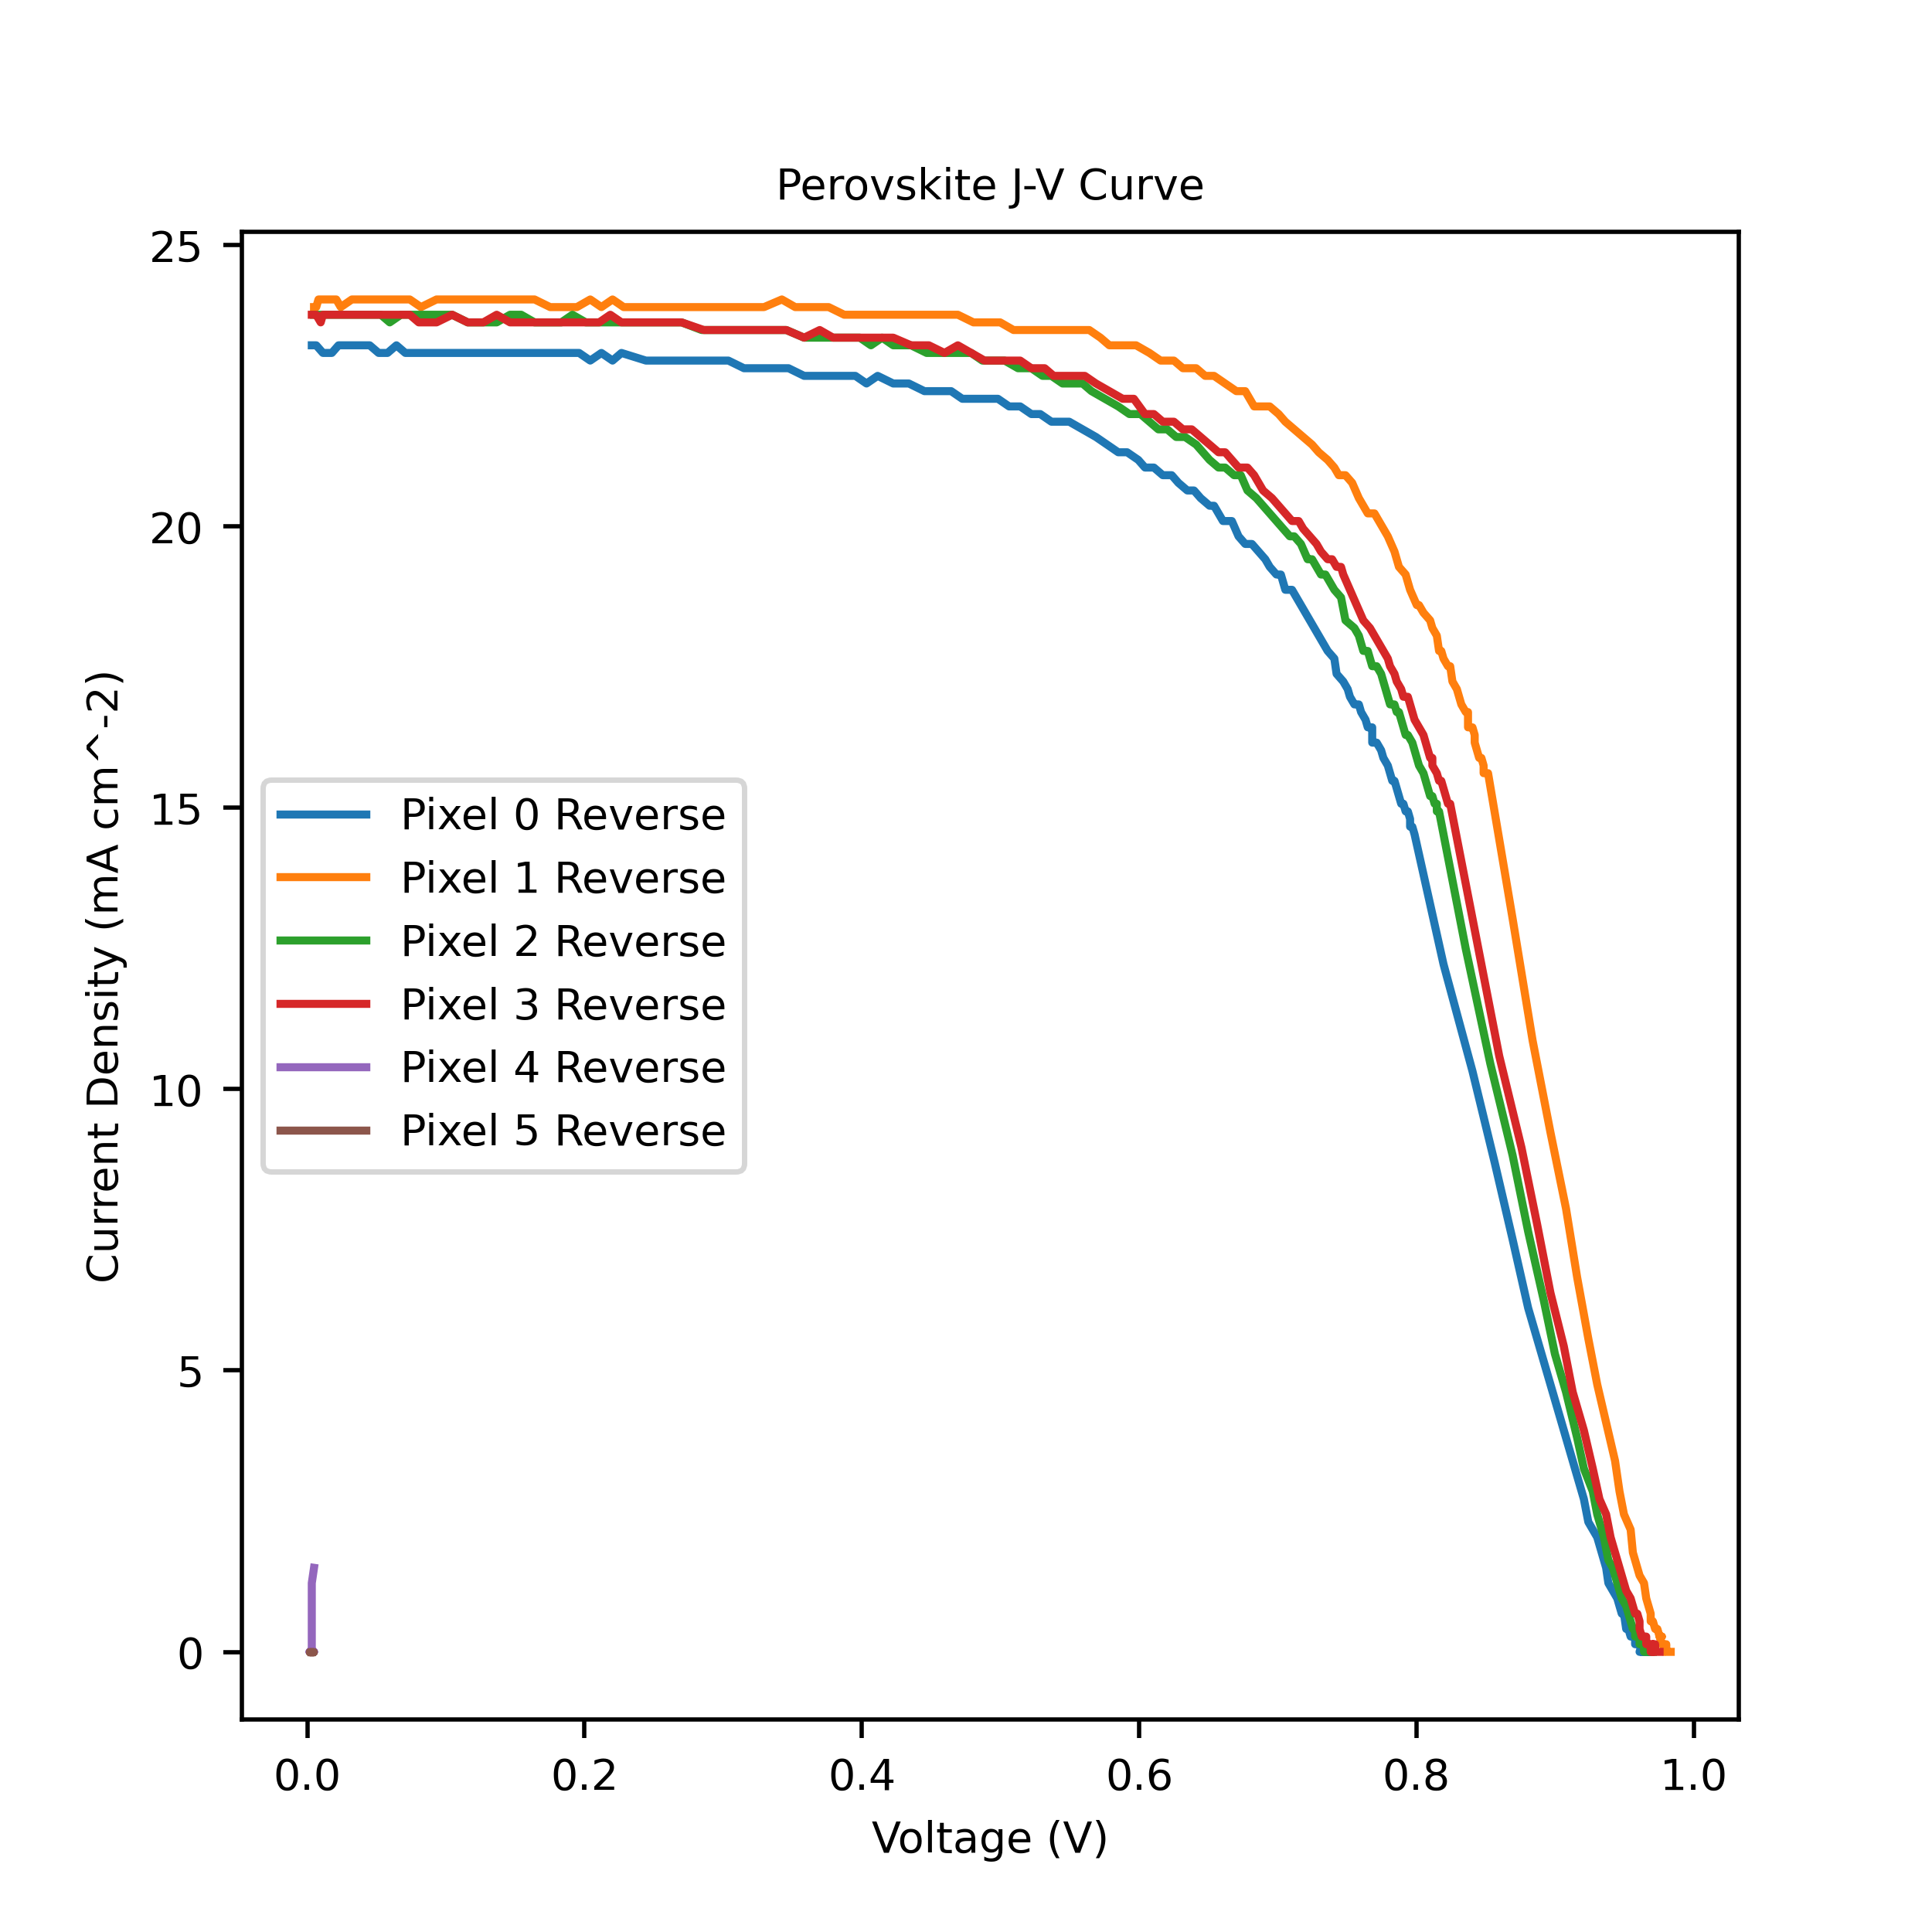
\includegraphics[width=8cm, height=7.5cm]{X017_LM_plotted_Reverse.png}
	\caption{The curve tracer in use with the Ossila solar simulator illuminating the sample.}
	\label{fig:curves}
\end{figure}


\section*{Discussion}

\section*{Conclusions}

\section*{Acknowledgments} 

\section*{Author contributions statement}

\section*{Competing interests} 

\printbibliography %Prints bibliography

\end{document}